\chapter{Introduction}

\section{Background}

\textbf{Transformer} is a deep learning architecture proposed in the 2017 paper \textit{Attention Is All You Need} \cite{vaswani2017attention}, developed initially for machine translation. The transformer architecture has literally transformed the whole deep learning community since its debut, with its multiple advantages, including:

\begin{enumerate}
    \item \textbf{Efficacy}: Transformers utilize \textit{multi-head attention mechanism}, which effectively captures global information while processing data.
    \item \textbf{Efficiency}: The design of Transformer (discarding recurrent networks) allows significant parallelization, which greatly speeds up model training and evaluation.
\end{enumerate}

To date, Transformer has not only gained tremendous success in NLP tasks (e.g. GPT-4 \cite{achiam2023gpt}), but has also been applied to modalities beyond text, including image/video generation (e.g. Sora \cite{videoworldsimulators2024}), computer vision (e.g. ViT \cite{dosovitskiy2020image}), and more. Here, we merely focus on NLP tasks for simplicity.

\section{Related Works}

In essence, the transformer architecture incorporates multiple past innovations, including attention mechanism, layer normalization, residual connection, etc.

Prior to the transformer architecture, attention mechanisms were primarily employed within sequence-to-sequence models \cite{bahdanau2014neural}. However, these attention mechanisms were typically constrained by the sequential processing imposed by RNNs, which severely limited opportunities for parallelization. In contrast, the transformer model \cite{vaswani2017attention} replaces recurrence with a self-attention mechanism. This innovative approach enabled parallel computation across the entire input sequence, leading to substantial improvements in training efficiency and scalability. 

Layer normalization is proposed in \cite{ba2016layer} to address the problems of batch normalization and acts as a method for normalization in RNNs. Residual networks, first appearing in \cite{he2016deep}, aim to solve training issues of deep neural networks, especially in CNNs. Both layer normalization and residual connections enable a more stable training process for transformers.

\section{Transformer Overview} \label{sec:transformer_overview}

The transformer architecture mainly consists of two components: (1) \textbf{embedding layers} (2) \textbf{transformer blocks}. An embedding layer maps input tokens (or simply, \textit{words}) to numerical representations, or vice versa. That is, input words are converted to numerical vectors (embeddings) for further processing. And after all calculations, those embeddings are converted back to textual data. The transformer blocks constitute the core of the overall architecture. A transformer block is composed of the following:

\begin{itemize}
    \item \textbf{an attention layer},
    \item \textbf{a feedforward layer},
    \item \textbf{layer normalizations (layer norms)}, and
    \item \textbf{residual connections}.
\end{itemize}

Figure \ref{fig:tranformer_atchitecture} illustrates the transformer architecture globally. In the following sections, we will first introduce the \textbf{attention mechanism} in Chapter \ref{chap:attention}. The other ingredients of the transformer block will be covered in Chapter \ref{chap:transformer}.

\begin{figure}
    \centering
    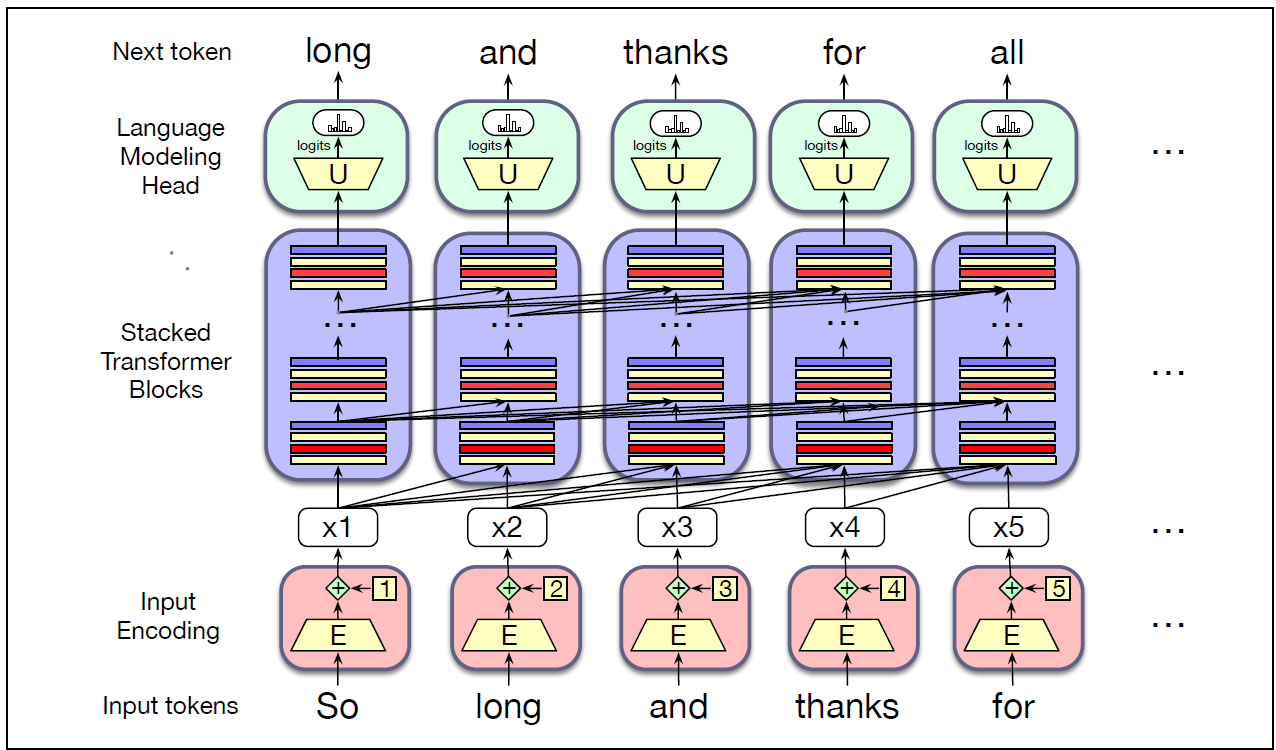
\includegraphics[width=1\linewidth]{fig/transformer_architecture.png}
    \caption{A (decoder-only) transformer model illustration for text generation \cite{jm3}.}
    \label{fig:tranformer_atchitecture}
\end{figure}